\documentclass[12pt]{article}

\usepackage{sbc-template}
\usepackage{graphicx}
\usepackage[utf8]{inputenc}
\usepackage[brazil]{babel}
% \usepackage{url}
\usepackage{amsmath}
\usepackage{amssymb}
\usepackage{float}
\usepackage[hyphens]{url}
% \PassOptionsToPackage{hyphens}{url}
% \usepackage{hyperref}

\sloppy

\title{Comparação de Estratégias de Ajuste Fino em LLMs de Pequeno Porte para Geração de Títulos Acadêmicos}

\author{Omitido para avaliação cega}

\address{Omitido para avaliação cega
  \email{omitido@omitido}
}

\begin{document}

\maketitle

\begin{resumo}
Este trabalho investiga a adaptação de LLMs de pequeno porte para geração automática de títulos científicos. Utilizando o modelo Qwen2,5-0,5B-Instruct e dados do arXiv, comparou-se Baseline, Fine-Tuning da última camada, Q-LoRA e Full Fine-Tuning. A performance foi avaliada via métrica S-BERT e análise qualitativa. Os resultados do teste de Kruskal-Wallis ($H=30,53$, $p<0,001$) indicaram diferenças significativas entre os métodos. O Treinamento Completo obteve o melhor desempenho, porém o Q-LoRA atingiu resultados estatisticamente equivalentes, validando sua eficiência. Em contrapartida, o ajuste da última camada mostrou-se inferior ao baseline. A análise qualitativa revelou que o modelo Q-LoRA apresenta maior instabilidade estrutural em arquiteturas compactas.
\end{resumo}

\begin{abstract}
This work investigates the efficient adaptation of small Large Language Models (LLMs) for automatic title generation from scientific abstracts. Using the Qwen2.5-0.5B-Instruct base model and arXiv data, four experimental approaches were compared: Baseline (zero-shot), Last-Layer Fine-Tuning, Q-LoRA, and Full Fine-Tuning. Performance was evaluated quantitatively using S-BERT semantic similarity and qualitatively through human analysis. Kruskal-Wallis test results ($H=30.53$, $p<0.001$) demonstrated significant differences between methods. Full Fine-Tuning achieved the best absolute performance, but the Q-LoRA method reached statistically equivalent results, validating its efficiency. Conversely, adjusting only the last layer proved inferior to the baseline. Qualitative analysis also indicated that the quantized model (Q-LoRA) exhibited greater structural instability, suggesting the sensitivity of compact architectures to quantization.
\end{abstract}

\section{Introdução}\label{sec:intro}



O crescimento exponencial da produção científica representa um desafio crescente para a descoberta e curadoria de conhecimento. Repositórios como o arXiv \cite{arxivorg_submitters_arxiv_nodate} acumulam milhões de artigos, com novos trabalhos submetidos diariamente em áreas como computação, física e matemática. Nesse contexto, sistemas capazes de gerar automaticamente metadados, como títulos e palavras-chave, a partir do conteúdo textual dos artigos têm aplicação direta em indexação, busca semântica e recomendação acadêmica.

Com o advento dos Grandes Modelos de Linguagem (LLMs), tornou-se possível abordar essa tarefa com qualidade sem precedentes. Entretanto, o emprego direto de LLMs pré-treinados sem especialização produz resultados inconsistentes: conforme observado neste estudo, o modelo sem ajuste fino gerou títulos excessivamente longos e com artefatos do \textit{prompt} de instrução, evidenciando a necessidade de especialização para a tarefa. O principal obstáculo ao ajuste fino em contextos com restrições computacionais é o custo proibitivo do treinamento completo, que exige o armazenamento de gradientes e estados do otimizador para todos os parâmetros do modelo. Métodos de ajuste fino com eficiência paramétrica (PEFT)~\cite{ding_parameter-efficient_2023}, como LoRA~\cite{hu_lora_2022} e Q-LoRA~\cite{dettmers_qlora_2023}, surgem como alternativas que reduzem drasticamente esse custo. Contudo, a comparação sistemática dessas estratégias em tarefas aplicadas de geração de texto com modelos de pequeno porte permanece pouco explorada na literatura.

Este trabalho investiga esse problema ao comparar quatro estratégias de adaptação (Baseline zero-shot, ajuste da última camada (\textit{Linear Probing}), Q-LoRA e \textit{Full Fine-Tuning}) aplicadas ao modelo Qwen2,5-0,5B-Instruct para a geração automática de títulos a partir de resumos do arXiv. Os resultados demonstram que o Q-LoRA alcança desempenho estatisticamente equivalente ao treinamento completo ($p = 0,109$), validando sua viabilidade como alternativa eficiente para pesquisadores e instituições com infraestrutura limitada.

A tarefa se assemelha à sumarização automática de textos, na qual um LLM processa um texto de entrada para retornar uma versão reduzida que preserva o sentido do conteúdo original. Entretanto, o objetivo difere ligeiramente: ao invés de produzir resumos, trata-se da geração de títulos a partir de resumos de artigos científicos. Esta tarefa apresenta desafios intrínsecos: é comum que autores optem por títulos ``chamativos'' ou estilizados que não podem ser diretamente inferidos a partir do resumo. Quando tais títulos são utilizados como \textit{ground truth} no treinamento, o modelo enfrenta dificuldades de convergência, pois a correlação semântica entre a entrada e a saída esperada é fraca.

Outro desafio crítico reside na métrica de avaliação. A comparação literal entre o título gerado e o original é insuficiente para capturar a qualidade da predição. Considere dois cenários de divergência: o título predito é uma permutação das palavras do título original; ou o título predito utiliza vocabulário distinto, mas com o mesmo significado semântico do original.

Para a aplicação proposta, o segundo caso é preferível, pois demonstra a capacidade do modelo de abstrair e sintetizar o conteúdo, em vez de apenas memorizar sequências de tokens. Torna-se necessário, portanto, empregar uma métrica que avalie a semelhança semântica. Uma abordagem amplamente adotada é o Sentence-BERT~\cite{reimers_sentence-bert_2019,devlin_bert_2019}, um modelo baseado em BERT treinado especificamente para medir similaridade semântica entre sentenças, gerando valores próximos de 0 para frases sem relação semântica e próximos de 1 para frases semanticamente equivalentes.

O restante deste artigo está organizado da seguinte forma. A Seção~\ref{sec:related} apresenta os trabalhos relacionados. A Seção~\ref{sec:metodologia} descreve a metodologia adotada, incluindo a construção do \textit{dataset} e as técnicas de treinamento avaliadas. A Seção~\ref{sec:experimento} detalha o protocolo experimental e as métricas de avaliação. A Seção~\ref{sec:resultados} apresenta e discute os resultados obtidos. Por fim, a Seção~\ref{sec:conclusao} sintetiza as conclusões e aponta direções para trabalhos futuros.

\section{Trabalhos Relacionados}\label{sec:related}


O paradigma de geração de texto condicionado consolidou-se com o modelo T5 (\textit{Text-to-Text Transfer Transformer})~\cite{raffel_exploring_2020}, que unificou tarefas diversas de PLN — sumarização, tradução e geração de respostas — em um único framework de entrada e saída textual, viabilizando o ajuste fino de modelos pré-treinados para tarefas de geração como a proposta neste trabalho. Brown et al.~\cite{brown_language_2020}, com o GPT-3, demonstraram que LLMs de grande escala podem realizar tarefas de geração via \textit{in-context learning} sem ajuste fino, mas também evidenciaram que, para domínios específicos, o zero-shot produz resultados inferiores aos obtidos com especialização supervisionada — observação corroborada pelo desempenho do \textit{baseline} neste estudo.

A arquitetura \textit{Transformer}~\cite{vaswani_attention_2017} e modelos derivados como o BERT~\cite{devlin_bert_2019} estabeleceram que representações contextualizadas pré-treinadas podem ser ajustadas para tarefas específicas com alta eficiência. O Sentence-BERT (S-BERT)~\cite{reimers_sentence-bert_2019} estende o BERT com uma rede siamesa para gerar \textit{embeddings} de sentenças comparáveis por similaridade semântica, tornando-se ferramenta padrão para avaliação de qualidade em geração de texto — papel que ocupa também neste trabalho.

Com o crescimento dos LLMs, o treinamento completo tornou-se computacionalmente inviável na maioria dos cenários práticos. Ding et al.~\cite{ding_parameter-efficient_2023} apresentam uma revisão sistemática dos principais métodos PEFT — adaptadores, \textit{prefix-tuning} e LoRA — demonstrando que o ajuste eficiente alcança desempenho comparável ao treinamento completo em tarefas de classificação e geração com uma fração dos parâmetros treináveis. O LoRA~\cite{hu_lora_2022} e sua extensão com quantização Q-LoRA~\cite{dettmers_qlora_2023} são os representantes mais utilizados desse paradigma, sendo ambos avaliados neste trabalho.

No contexto nacional, Souza et al.~\cite{souza_bertimbau_2020} demonstraram que o pré-treinamento adicional do BERT em corpora de português brasileiro (BERTimbau) gera ganhos significativos em tarefas como reconhecimento de entidades nomeadas e similaridade textual em relação a modelos multilíngues, evidenciando que a especialização de modelos pré-treinados em um domínio ou idioma é necessária para maximizar o desempenho. Esse princípio motiva diretamente a avaliação de estratégias de ajuste fino conduzida neste trabalho, agora aplicado ao domínio de textos científicos em inglês do arXiv.

Os modelos Qwen2~\cite{yang_qwen2_2024} e Qwen2.5~\cite{team_qwen25_2024} integram a nova geração de LLMs abertos com arquitetura eficiente, apresentando resultados competitivos em benchmarks de compreensão e geração de texto mesmo nas versões de menor porte. Estudos recentes sobre os efeitos da quantização em LLMs~\cite{shi_systematic_2025} indicam que, embora reduza custos computacionais, a quantização pode introduzir degradação de qualidade variável dependendo da tarefa e da arquitetura — aspecto diretamente relevante para a interpretação dos resultados obtidos com o Q-LoRA neste estudo.


\section{Metodologia}\label{sec:metodologia}

\subsection{Construção do Dataset}\label{subsec:dataset}



Os dados utilizados neste estudo foram obtidos a partir do repositório público do arXiv \cite{arxivorg_submitters_arxiv_nodate}. O \textit{dataset} original é distribuído no formato JSON e contém os seguintes campos: \texttt{id}, \texttt{submitter}, \texttt{authors}, \texttt{title}, \texttt{comments}, \texttt{journal-ref}, \texttt{doi}, \texttt{report-no}, \texttt{categories}, \texttt{license}, \texttt{abstract}, \texttt{versions}, \texttt{update\_date} e \texttt{authors\_parsed}.

Para o escopo deste trabalho, utilizou-se apenas os campos \texttt{abstract} (resumo) e \texttt{title} (título). Uma análise exploratória preliminar dos dados revelou a presença de sequências textuais extensas: o maior \texttt{abstract} registrado possui 6.091 caracteres, enquanto o título mais longo contém 382 caracteres. Essas métricas são relevantes pois impactam diretamente a escolha da janela de contexto do modelo de linguagem.

O pré-processamento dos dados para o \textit{fine-tuning} envolveu uma estratégia de subamostragem aleatória (random subsampling), visando a viabilidade computacional. Foram gerados dois subconjuntos disjuntos: \begin{itemize} \item Conjunto de Treinamento: Composto por 10.000 amostras; \item Conjunto de Teste: Composto por 1.000 amostras. \end{itemize}

Na modelagem, o atributo \texttt{abstract} foi utilizado como variável de entrada do modelo, enquanto o atributo \texttt{title} foi adotado como alvo. Assim, o objetivo do treinamento é que o modelo seja capaz de gerar, a partir do resumo, um título que seja semanticamente equivalente ao conteúdo presente no atributo title.

\subsection{Técnicas de Treinamento}\label{subsec:treinamento}



Para a adaptação do modelo de linguagem à tarefa de geração de títulos, foram exploradas três abordagens distintas: (i) \textit{Baseline} (sem treinamento); (ii) \textit{Fine-tuning} da última camada; e (iii) \textit{Fine-tuning} eficiente via Q-LoRA.

\subsubsection{Quantized Low-Rank Adaptation (Q-LoRA)}

O método Q-LoRA~\cite{dettmers_qlora_nodate} é uma extensão da técnica LoRA~\cite{hu_lora_2022} (Low-Rank Adaptation), otimizada para eficiência de memória. Enquanto o LoRA congela os pesos pré-treinados do modelo e injeta pares de matrizes de decomposição de posto (rank) reduzido em cada camada, o Q-LoRA introduz a quantização dos pesos do modelo base para 4-bits (formato \textit{NormalFloat4}), mantendo os adaptadores treináveis em precisão mista (e.g., \textit{BFloat16}).

Matematicamente, para uma camada linear pré-treinada com pesos $W_0 \in \mathbb{R}^{d \times k}$, a atualização dos pesos $\Delta W$ é parametrizada por uma decomposição de baixo posto $BA$, onde $B \in \mathbb{R}^{d \times r}$ e $A \in \mathbb{R}^{r \times k}$, sendo $r \ll \min(d, k)$ o posto (rank) da adaptação. A operação de \textit{forward pass} é então expressa como:

\begin{equation}
h = W_0 x + \Delta W x = W_0 x + B A x
\end{equation}
Onde $x$ é o vetor de entrada e $h$ o vetor de saída.

A principal vantagem reside na eficiência paramétrica. O número de parâmetros treináveis ($N_{LoRA}$) em comparação com o treinamento completo ($N_{Full}$) é dado pela relação entre as dimensões das matrizes. Para que haja redução de parâmetros, a seguinte desigualdade deve ser satisfeita:

\begin{equation}
    \underbrace{d \times r + r \times k}_{N_{LoRA}} \ll \underbrace{d \times k}_{N_{Full}}
\end{equation}

Simplificando para o caso onde as dimensões de entrada e saída são iguais ($d=k$):\begin{equation}2dr \ll d^2 \implies 2r \ll d\end{equation}Como $d$ (dimensão oculta do modelo) cresce linearmente e $d^2$ quadraticamente, existe um amplo intervalo para $r$ que garante uma redução drástica na contagem de parâmetros, viabilizando o treinamento em hardwares com memória limitada.

É importante notar que, embora o armazenamento seja reduzido, a inferência direta com LoRA introduz uma latência computacional adicional, pois requer duas multiplicações matriciais extras ($Wx + BAx$). Esse custo pode ser eliminado através da técnica de \textit{Weight Merging}, onde as matrizes $A$ e $B$ são multiplicadas e somadas aos pesos originais ao final do treinamento ($W' = W_0 + BA$), restaurando a arquitetura original do modelo sem custos adicionais de latência.

\subsubsection{Fine-tuning da Última Camada}

A abordagem de \textit{Last-Layer Fine-Tuning} (ou \textit{Linear Probing}) restringe a atualização dos pesos (via \textit{backpropagation}) exclusivamente à camada de saída do modelo. Neste cenário, todas as camadas ocultas do \textit{Transformer}~\cite{vaswani_attention_2017} permanecem congeladas, funcionando apenas como extratoras de características. Embora computacionalmente eficiente, esta técnica limita a plasticidade do modelo em adaptar suas representações internas a novos domínios.

\subsubsection{Full Fine-Tuning (Treinamento Completo)}

A abordagem de Full Fine-Tuning (FFT) consiste na atualização irrestrita de todos os parâmetros $\theta$ do modelo pré-treinado durante o processo de aprendizado supervisionado. Diferente dos métodos PEFT (Parameter-Efficient Fine-Tuning), onde apenas um subconjunto de pesos ou adaptadores é ajustado, o FFT permite que a rede neural reconfigure todas as suas camadas ocultas e mecanismos de atenção para se adaptar à distribuição do novo dataset.

Embora esta técnica ofereça, teoricamente, a maior plasticidade e potencial de desempenho, ela impõe um custo computacional severo. O consumo de memória VRAM é significativamente maior, pois é necessário armazenar os estados do otimizador e os gradientes para a totalidade dos parâmetros do modelo (neste caso, 0.5 bilhões de parâmetros). Esta abordagem serve, portanto, como o ``padrão-ouro'' para comparação com as técnicas de eficiência.

\subsubsection{Modelo Baseline e Prompting}

O modelo base adotado para todos os experimentos foi o Qwen2.5-0.5B-Instruct~\cite{yang_qwen2_2024,team_qwen25_2024}.
A escolha deste modelo justifica-se pelo seu tamanho compacto (0,5 bilhões de parâmetros), permitindo iterações rápidas de experimentação, com poucos recursos computacionais.

Para o treinamento supervisionado, os dados foram estruturados utilizando o formato de template \textit{ChatML}, conforme ilustrado abaixo:

\begin{verbatim}
<|im_start|>system
You are a specialist in suggesting titles based on the abstract.
<|im_end|>

<|im_start|>user
{exemplo['abstract']}
<|im_end|>

<|im_start|>assistant
{exemplo['title']}{EOS_TOKEN}
\end{verbatim}

Este prompt delimita claramente as instruções do sistema, a entrada do usuário (resumo) e a saída esperada (título), facilitando com que o modelo seja treinado como um especialista na geração de títulos a partir de resumos. O usuário deve apenas fornecer o resumo do artigo para que o modelo produza um título adequado.



% A principal vantagem desse método reside na redução do parâmetro $k$, uma vez que, quanto menor for seu valor, menor será o número de parâmetros que precisam ser ajustados. Considere a seguinte relação:

% \begin{align*}
% A \times k + B \times k & \le A \times B \\
% k (A + B) &\le A \times B \\
% k &\le \frac{A \times B}{A + B} \\
% \end{align*}

% Se $A$ e $B$ crescerem linearmente, o numerador aumentará em ordem quadrática, enquanto o denominador crescerá em ordem linear. Dessa forma, existe um amplo intervalo de valores possíveis para $k$ que ainda garante uma quantidade de parâmetros significativamente menor do que aquela necessária para treinar toda a camada.

% Entretanto, após o treinamento, ainda é necessário incorporar as matrizes adaptadas à rede original. Além disso, embora o número de parâmetros treináveis seja reduzido, a fase de inferência (tanto no treinamento quanto no teste) passa a envolver mais parâmetros devido à presença das matrizes adicionais, o que pode tornar o modelo maior e potencialmente mais lento nessa etapa. Esses efeitos podem ser mitigados se, ao final do treinamento, as contribuições aprendidas nas matrizes $A$ e $B$ forem fundidas nas camadas originais do modelo, eliminando as estruturas auxiliares do LoRA e preservando os ganhos de eficiência obtidos durante o processo de treinamento.

% O fine-tuning da última (ou mais) camadas consiste de permitir que o valor dos parâmetros seja ajustado durante o treinamento. Embora, isso tenha impactos em termos de performance, não há mudanças além do treinamento comum usando backpropagation.

% O baseline utilizado neste trabalho foi o modelo original, isto é, o modelo Qwen2.5-0.5B-Instruct~\cite{yang_qwen2_2024,team_qwen25_2024}.

% O prompt usado para treinar o modelo foi o seguinte:

% \begin{verbatim}
% <|im_start|>system
% You are a specialist in suggesting titles based on the abstract.
% <|im_end|>

% <|im_start|>user
% {exemplo['abstract']}
% <|im_end|>

% <|im_start|>assistant
% {exemplo['title']}{EOS_TOKEN}
% \end{verbatim}

% Neste prompt, o modelo é treinado como um especialista na geração de títulos a partir de resumos. O usuário deve apenas fornecer o resumo do artigo para que o modelo produza um título adequado.


\section{Experimentos}\label{sec:experimento}



Os experimentos foram desenhados para avaliar comparativamente o desempenho do modelo nos quatro cenários metodológicos descritos na Seção 3:

\begin{itemize}
    \item M1 - \textit{Baseline}: Inferência direta sem treinamento (\textit{Zero-shot});
    \item M2 - \textit{Last-Layer Fine-Tuning}: Ajuste fino restrito à camada de saída;
    \item M3 - Q-LoRA: Ajuste fino eficiente com quantização 4-bit.
    \item M4 - \textit{Full Fine-Tuning}: Atualização de todos os parâmetros do modelo pré-treinado.
\end{itemize}

Os modelos submetidos ao fine-tuning (M2, M3 e M4) foram treinados em uma base de dados composta por 10 mil amostras selecionadas aleatoriamente, conforme detalhado na Seção 2. O conjunto completo não foi utilizado devido a limitações computacionais.

A validação dos resultados foi conduzida através de duas abordagens complementares: avaliação automática (quantitativa) e avaliação humana (qualitativa).

\subsection{Avaliação Automática (S-BERT)}

O objetivo do experimento é identificar qual modelo apresenta o melhor desempenho na geração de títulos. A performance foi mensurada através da proximidade semântica entre o título gerado ($T_{gen}$) e o título original de referência ($T_{ref}$), utilizando a métrica S-BERT~\cite{reimers_sentence-bert_2019,zhang_semantics-aware_2020}.
Esta métrica calcula a similaridade de cosseno entre os embeddings das sentenças, sendo mais robusta a paráfrases do que métricas baseadas em n-gramas (como ROUGE ou BLEU).

\subsection{Avaliação Humana}

Para mitigar as limitações das métricas automáticas, realizou-se uma análise qualitativa em caráter exploratório. Dois avaliadores independentes responderam a um formulário contendo $8$ questões.
Cada item do formulário apresentava o resumo (\textit{abstract}) de um artigo seguido por cinco opções de títulos, apresentadas em ordem aleatorizada e sem qualquer identificação da técnica geradora (avaliação cega, \textit{blind evaluation}):

\begin{enumerate}
    \item O título original do autor (\textit{Ground Truth});
    \item O título gerado pelo \textit{Baseline} (M1);
    \item O título gerado pelo \textit{Last-Layer Fine-Tuning} (M2);
    \item O título gerado pelo Q-LoRA (M3).
    \item O título gerado pelo \textit{Full Fine-Tuning} (M4).
\end{enumerate}

Os avaliadores identificaram qual título melhor representava o conteúdo do resumo, considerando critérios de coerência semântica, concisão e correção gramatical. O protocolo de avaliação cega garante que as preferências registradas sejam independentes do conhecimento prévio sobre os métodos comparados.


\section{Resultados e Discussões}\label{sec:resultados}



% \input{sections/04.resultados}

% \section{Análise dos resultados}



A Figura~\ref{fig:training} apresenta a distribuição (\textit{boxplot}) e a média com desvio-padrão do \textit{SBERT-score} avaliado no conjunto de teste para os quatro experimentos. Esta métrica calcula a similaridade de cosseno entre os \textit{embeddings} das sentenças, operando teoricamente no intervalo $[-1, 1]$, onde valores próximos a $1$ indicam alta equivalência semântica entre os títulos gerado e de referência.

Os resultados evidenciam uma hierarquia de desempenho coerente com a capacidade de adaptação de cada método. O modelo com treinamento completo (M4) obteve a maior média de \textit{SBERT-score} ($\mu = 0,640$), seguido pelo Q-LoRA (M3) com $\mu = 0,627$. Notavelmente, o ajuste isolado da última camada (M2, $\mu = 0,596$) ficou aquém do \textit{baseline} sem treinamento (M1, $\mu = 0,614$). Esse resultado contraintuitivo pode ser explicado pelo fato de que, ao atualizar apenas a camada de saída mantendo os pesos intermediários congelados, o modelo não desenvolve representações internas adequadas à tarefa, introduzindo um desalinhamento entre as características extraídas pelas camadas ocultas e o comportamento esperado na decodificação.

\begin{figure}[!h]
    \centering
    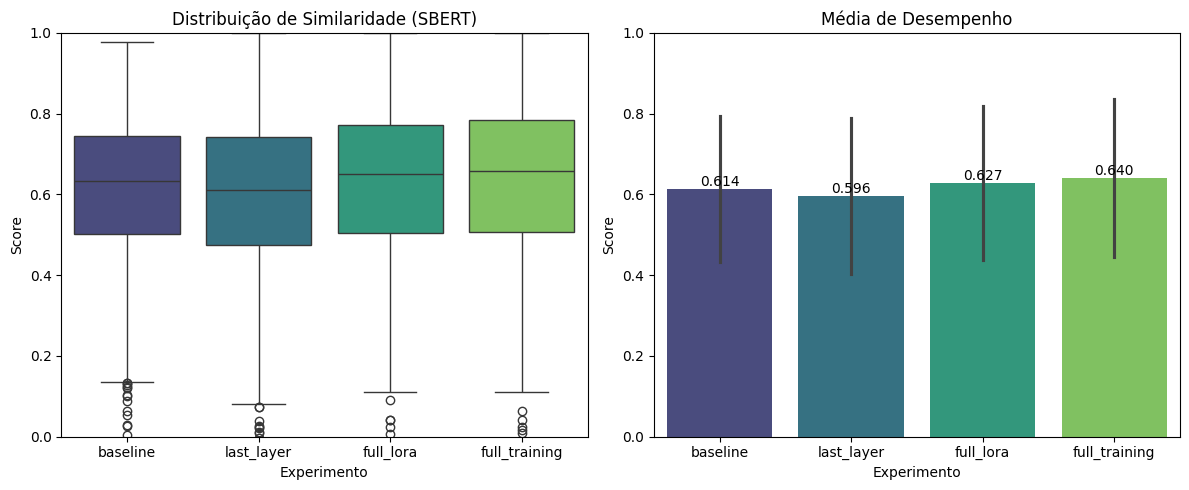
\includegraphics[width=1\linewidth]{figs/training_result.png}
    \caption{Distribuição do \textit{SBERT-score} no conjunto de teste para os quatro métodos avaliados. As caixas representam o intervalo interquartil (IQR) e os losangos indicam as médias amostrais.}
    \label{fig:training}
\end{figure}

Para verificar se as diferenças observadas nas médias são estatisticamente significativas, aplicou-se o teste não-paramétrico de Kruskal-Wallis. A escolha deste teste justifica-se pela violação da premissa de normalidade na distribuição dos \textit{scores} de similaridade, tornando inapropriado o uso de testes paramétricos como a ANOVA. A hipótese nula ($H_0$) postula que as medianas populacionais de todos os grupos são iguais.

O teste global resultou em $H = 30,53$ ($p < 0,001$), rejeitando $H_0$ com alto grau de confiança e confirmando que ao menos um par de métodos apresenta distribuições de desempenho significativamente distintas.

Para identificar quais pares de métodos diferem entre si, aplicou-se o teste \textit{post-hoc} de Mann-Whitney com correção de Bonferroni (nível de significância ajustado $\alpha \approx 0,0083$). Os resultados são apresentados na Tabela~\ref{tab:comparacao_treinamento}.


\begin{table}[H]
\centering
\begin{tabular}{l c c c}
\hline
\textbf{Comparação} & \textbf{Diferença Média} & \textbf{P-valor} & \textbf{Significativo?} \\
\hline
Full Training (M4) vs. Q-LoRA (M3)     & 0,0129 & 0,11    & Não \\
Full Training (M4) vs. Baseline (M1)   & 0,0268 & $<$0,001 & Sim \\
Full Training (M4) vs. Last-Layer (M2) & 0,0447 & $<$0,001 & Sim \\
Q-LoRA (M3) vs. Baseline (M1)          & 0,0138 & 0,08    & Não \\
Q-LoRA (M3) vs. Last-Layer (M2)        & 0,0318 & $<$0,001 & Sim \\
Baseline (M1) vs. Last-Layer (M2)      & 0,0179 & 0,04    & Não$^{*}$ \\
\hline
\end{tabular}
\caption{Resultados do teste \textit{post-hoc} de Mann-Whitney com correção de Bonferroni ($\alpha \approx 0,0083$). $^{*}$Diferença tendencialmente significativa ($p < 0,05$), porém não confirmada após o ajuste para comparações múltiplas.}
\label{tab:comparacao_treinamento}
\end{table}

A análise dos resultados permite extrair três conclusões principais. Primeiramente, a superioridade do treinamento completo sobre métodos fracos foi confirmada, pois o M4 superou estatisticamente tanto o \textit{baseline} quanto o ajuste da última camada ($p < 0,001$ em ambos os casos), ratificando que a atualização irrestrita dos parâmetros é a estratégia mais eficaz para a tarefa estudada. Em segundo lugar, verificou-se a equivalência entre Full Fine-Tuning e Q-LoRA, uma vez que a comparação entre M4 e M3 resultou em $p = 0,109$, indicando ausência de diferença estatisticamente significativa. Este é o achado central do trabalho: o Q-LoRA, que demanda uma fração dos recursos computacionais do treinamento completo, alcança desempenho estatisticamente equivalente ao método mais custoso, validando sua eficiência como alternativa PEFT para cenários com restrições de infraestrutura. Por fim, notou-se a inadequação do ajuste isolado da última camada, visto que a comparação entre M2 e M1 resultou em $p = 0,04$, o qual não é estatisticamente significativo após a correção de Bonferroni.

Para complementar a avaliação quantitativa e mitigar as limitações das métricas automáticas — que podem não capturar aspectos como fluência, concisão e adequação estilística —, realizou-se uma análise qualitativa exploratória. Dois avaliadores independentes classificaram, em caráter cego, os títulos gerados pelos quatro modelos em oito amostras aleatórias do conjunto de teste. O design de avaliação cega reduz o viés de confirmátorio e fortalece a validade interna das observações. As principais observações indicaram verbosidade e artefatos no Baseline (M1), no qual o modelo sem treinamento demonstrou compreensão do conteúdo do resumo, mas produziu consistentemente títulos excessivamente longos e explicativos, com artefatos provenientes do prompt de instrução. Quanto ao Last-Layer Fine-Tuning (M2), observou-se degradação semântica, corrigindo parcialmente a extensão mas introduzindo erros semânticos sutis e instâncias de alucinação de termos técnicos. Por outro lado, notou-se alta fidelidade no Q-LoRA (M3) e Full Fine-Tuning (M4), onde ambos os modelos produziram títulos fluentes, concisos e semanticamente adequados na grande maioria das amostras, com o M4 destacando-se pela precisão terminológica e o M3 apresentando raros casos de inserção de contexto externo.

Em síntese, a avaliação qualitativa corrobora os achados quantitativos: o Full Fine-Tuning (M4) representa o teto de desempenho absoluto, enquanto o Q-LoRA (M3) constitui a alternativa de maior custo-benefício, com qualidade textual praticamente indistinguível na maioria dos casos analisados. A instabilidade pontual observada no M3 sugere um efeito colateral da quantização agressiva em modelos de pequeno porte, fenômeno que merece investigação aprofundada em trabalhos futuros.


% Dada a equivalência nas métricas automáticas, a avaliação humana tornou-se crítica para diferenciar os modelos. A análise foi conduzida sobre uma amostra aleatória de 8 instâncias do conjunto de teste, nas quais foram comparados o título original e os títulos gerados por M1, M2 e M3.

% As principais observações foram:

% \begin{itemize}
%     \item \textbf{Concisão do M2:} Embora M1 e M2 tenham gerado resultados semanticamente próximos, o modelo com ajuste da última camada (M2) demonstrou uma tendência a gerar títulos mais concisos e diretos, adequando-se melhor ao estilo acadêmico.
%     \item \textbf{Degradação Estrutural do M3:} O modelo treinado com Q-LoRA apresentou alucinações estruturais, gerando, em alguns casos, listas de tópicos ao invés de um título declarativo único.
% \end{itemize}

% A queda qualitativa perceptível no M3, apesar de manter a média semântica, sugere um efeito colateral da quantização agressiva (4-bits) em modelos de menor porte ($0.5$B parâmetros), que possuem menor redundância para absorver a perda de precisão numérica.


\section{Conclusão}\label{sec:conclusao}



Este trabalho investigou estratégias de adaptação eficiente de LLMs de pequeno porte para a tarefa de geração automática de títulos científicos a partir de resumos, utilizando o modelo Qwen2,5-0,5B-Instruct e um subconjunto de 10.000 amostras do repositório arXiv. Quatro abordagens foram comparadas: \textit{Baseline} zero-shot (M1), ajuste da última camada --- \textit{Linear Probing} (M2), Q-LoRA (M3) e \textit{Full Fine-Tuning} (M4).

Os resultados obtidos por meio da métrica S-BERT e corroborados pela avaliação qualitativa humana permitem responder à questão central do estudo com clareza. O \textit{Full Fine-Tuning} (M4, $\mu = 0,640$) representa o teto de desempenho absoluto, superando estatisticamente o \textit{baseline} e o ajuste da última camada ($p < 0,001$). O método Q-LoRA (M3, $\mu = 0,627$), contudo, alcançou desempenho estatisticamente equivalente ao M4 ($p = 0,109$), com qualidade textual praticamente indistinguível na avaliação humana, o que valida sua eficiência como alternativa PEFT em cenários com restrições computacionais. Em contrapartida, o ajuste isolado da última camada (M2, $\mu = 0,596$) produziu desempenho inferior ao do modelo original sem treinamento, evidenciando que a atualização de um único componente da rede, sem ajuste das representações intermediárias, é insuficiente para esta tarefa.

Outro achado relevante é a maior variância observada nos resultados do Q-LoRA em relação ao \textit{Full Fine-Tuning}, manifestada qualitativamente como inserção esporádica de contexto externo nos títulos gerados. Esse comportamento sugere uma sensibilidade de modelos compactos à quantização de 4 bits, que, ao reduzir a redundância paramétrica disponível, pode comprometer a estabilidade gerativa mesmo quando a média de desempenho permanece competitiva.

Como limitação, ressalta-se que os experimentos foram conduzidos com um único modelo de pequeno porte (0,5B parâmetros) e com uma amostra restrita do conjunto de dados, em razão de restrições computacionais. Trabalhos futuros poderão expandir esta investigação avaliando modelos de maior escala (e.g., 1,5B e 7B parâmetros) e diferentes níveis de quantização (4-bit vs.\ 8-bit), a fim de determinar o limiar de compressão aceitável e verificar se a instabilidade observada no M3 é um fenômeno específico de arquiteturas compactas. A literatura recente aponta esta como uma direção promissora: Egashira et al.~\cite{egashira_exploiting_nodate} e Shi e Ding~\cite{shi_systematic_2025} caracterizam sistematicamente os impactos da quantização sobre desempenho, consumo energético e consistência de geração em LLMs, reforçando a necessidade de estudos controlados sobre o tema.

\section*{Declaração de Ética}
Esta pesquisa utiliza documentos públicos e não envolve dados pessoais ou sensíveis. Todos os procedimentos seguiram os padrões éticos aplicáveis.

\section*{Uso de IA Generativa}
Ferramentas de IA generativa foram utilizadas para auxiliar na revisão linguística e no refinamento do texto. Todo o conteúdo científico, o desenho experimental e a análise foram conduzidos pelos autores.

\bibliographystyle{sbc}
\bibliography{references}

\end{document}
